
\section{Anforderungsspezifikation}


\subsection{Einf"uhrung}


\begin{itemize}
    \item requirement
    \item traceability
\end{itemize}


\subsubsection{Anforderung und Spezifikation}

\textbf{Anforderungen} sind eine Bedingung oder F"ahigkeit, die von einer Person zur L"osung eines Problems oder zur Erreichung eines Ziels ben"otigt wird.

\textbf{Softwareanforderungen} sind eine Bedingung oder F"ahigkeit, die eine Software erf"ullen oder besitzen muss, um einen Vertrag, eine Norm oder ein weiteres formelles Dokument zu erf"ullen.


\textbf{Muss-Anforderungen:}
\begin{itemize}
    \item unverzichtbar
    \item z.B. maximale Reaktionszeit
\end{itemize}

\textbf{Soll-Anforderungen:}
\begin{itemize}
    \item wichtig, aber bei zu hohen Kosten verzichtbar
    \item z.B. Online-"Uberpr"ufung von Benutzereingaben, internen Berechnungen oder Kommunikationsdaten
\end{itemize}

\textbf{Wunsch-Anforderungen:}
\begin{itemize}
    \item sch"on zu haben, aber nicht essenziell
    \item z.b. automatisches Update
\end{itemize}


Eine \textbf{Softwarespezifikation} ist eine Zusammenstellung aller Anforderungen an eine Software und der Randbedingungen f"ur ihren Einsatz.\\
Auch bekannt als: Software-Anforderungsspezifikation und Software-Anforderungsdokument.\\
Aufgabe der Spezifikation ist es, die angestrebte Diensterbringung zu beschreiben.\\
Es ist \textbf{nicht} das Ziel L"osungsans"atze zur Problemstellung beschreiben.

\subsubsection{Functionale vs. nicht-funktionale Anforderungen}

\textbf{Funktionale Anforderungen} beschreiben die Dienste, die die Software erbringen soll, also zum erw"unschten Verhalten der Software in bestimmten Situationen.\\
\textbf{Nicht-funktionale Anforderungen} sind weitere Einschr"ankungen der durch die Software zu erbringenden Dieste.



\subsubsection{Zentrale rolle der Spezifikation}
Vereinbarungen zwischen Auftraggeber und Entwickler (Pflichtenheft)
\begin{itemize}
    \item Vermeiden von Missverst"andnissen
    \item Detaillierte Bewschreibung des Funktionsmumfangs
    \item Eindeutiges Formulieren von Softwareeigenschaften
    \item Vertragscharakter
\end{itemize}

Abnahmetest
\begin{itemize}
    \item Soll klar definiert werden
    \item Vorteil f"ur Auftraggeber und Entwickler
\end{itemize}

\subsubsection{Eigenschaften von Anforderungen}
Jede Anforderung muss
\begin{itemize}
    \item Vollst"andigkeit
    \item Konsistenz
    \item Korrektheit
    \item Eindeutigkeit
    \item Realisierbarkeit
    \item Verfolgbarkeit
    \item Nachweisbarkeit
\end{itemize}
sein.\\

Anforderungen m"ussen die zu erbringende Funktionalit"at \textbf{vollst"andig} beschreiben, d.h., 
\begin{itemize}
    \item alle m"oglichen Eingaben oder Klassen von Eingabewerten und potenziell eintreffende Ereignisse sind inklusive der m"oglichen Kombinationen zu betrachten.
    \item Zudem muss die gew"unschte Reaktion des Systems detailliert beschrieben werden.
\end{itemize}

Jede einzelne Anforderung muss in sich selbst \textbf{konsitent} sein, d.h. \textbf{widerspruchsfrei}, sein.\\
Jede Anforderung ist \textbf{korrekt}, wenn sie die Absicht des Auftraggebers vollst"andig und konsistent wiedergibt.\\
Jede Anfroderung ist \textbf{eindeutig}, wenn sie nur auf eine Art und Weise interpretiert werden kann.\\
Eine Anforderung ist \textbf{realisierbar}, wenn es m"oglich ist, die Anforderung unter den im voraus bekannten \textbf{Randbedingungen} (u.a. an den Software-Entwicklungsprozess), mit R"ucksicht auf die \textbf{Grenzen des Systems} und seiner Umgebung in ein ablauff"ahiges System umzusetzen.\\
Eine Anforderung ist \textbf{verfolgbar}, wenn
\begin{itemize}
    \item sie eindeutig \textbf{identifizierbar} ist
    \item ihre schrittweise Umsetzung durch den gesamten Software-Lebenszyklus \textbf{durchg"angig auffindbar} ist.
\end{itemize}
Eine Anforderug ist \textbf{nachweisbar}, wenn eindeutige Kriterien zur "Uberpr"ufung ihrer Erf"ullung existieren.\\


\subsection{Allgemeine Anforderungsermittlung}

\subsubsection{Anforderungsermittlung}

Requirements Engineeri8ng ist auch immer
\begin{itemize}
    \item Aufgabenkl"arung
    \item Konsensbildung
    \item Konflikterkennung und -aufl"osung
\end{itemize}
Allgemeine Vorgehensweise
\begin{itemize}
    \item Problemdefinition
    \item Identifizieren der Stakeholder
    \item Ermitteln der Anforderungen und Festlegen der Systemgrenzen
\end{itemize}

\subsubsection{Problemdefinition}
\textbf{Einigung} "uber das Problem, das gel"ost werden soll.\\
\textbf{Beschreibung} der Problemdefinition aus der Sicht des Anwenders.\\

\subsubsection{Identifizieren der Stakeholder}
Stakeholders sind alle Personen, die von der \textbf{Systementwicklung und vom Einsatz und Betrieb des Systems betroffen sind}, also insbesondere Personen die das System nutzen, in Betrieb halten oder schulen.\\


\subsubsection{Ermitteln der Anforderungen}
Techniken:
\begin{itemize}
    \item Brainstormin
    \item Fragebogen
    \item Interview
    \item Simulationsmodelle (z.B. Prototyping)
    \item Anforderungsreview
    \item Workshop
\end{itemize}

\subsubsection{Konkrete Vorgehensweise}

Vorgehensweise zur Entwicklung einer Spezifikation am Beispiel des \textbf{Volere-Modells}.\\
\begin{description}
    \item[Schritt 1] Anwendungsfallmodellierung
    \item[Schritt 2] Festhalten der Anforderungen
    \item[Schritt 3] Zusammenstellen der Spezifikation
\end{description}

\subsubsection{Anwendungsfalldiagramm}
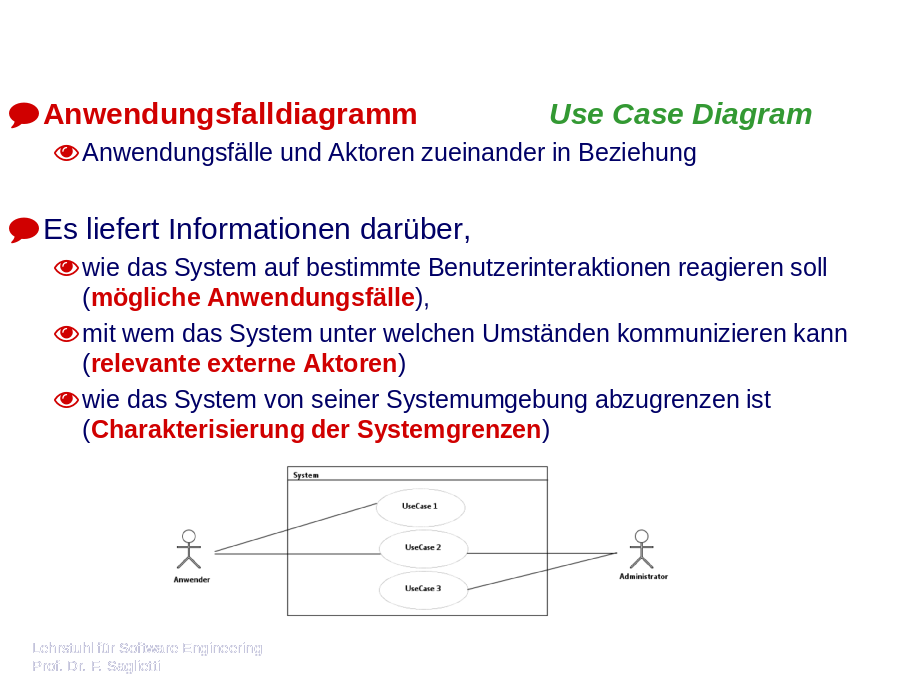
\includegraphics[scale=0.5]{./inc/Anforderungsspezifikation/UseCaseDiagram.png}

\subsubsection{Festhalten der Anforderungen}
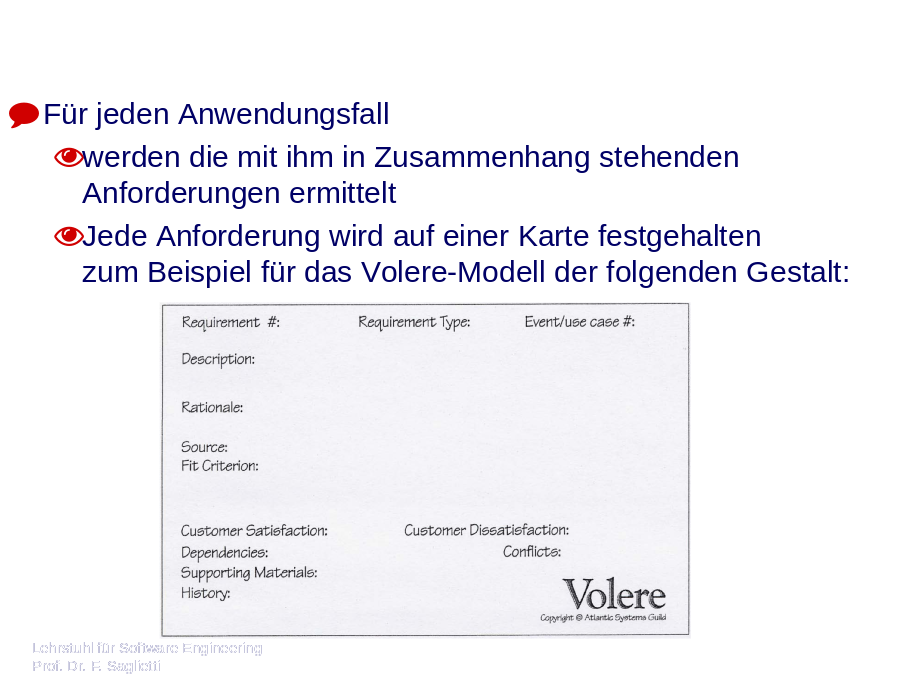
\includegraphics[scale=0.5]{./inc/Anforderungsspezifikation/Anforderungskarten.png}

\begin{description}
    \item[Anforderungsnummer] Jede Anforderung wird eindeutig durchnummeriert
    \item[Anwendungsfallnummer] Verweis auf einen Anwendugnsfall bzq. auf mehrere Anwendungsf"alle (dadurch implizit betroffene Anwernder festgelegt
    \item[Beschreibung der Anforderung] formuliert in der Sprache des Anwenders
    \item[Motivation] Der Grund f"ur diese Anforderung. (Warum ist diese Anforderung wichtig?)
    \item[Urheber] Name der Person, die diese Anforderung gestellt hat
    \item[Abnahmekriterien] Akzeptantz-Kriterien f"ur Abnahmetest
    \item[Kundenzufriedenheit] Gef"uhl von Freude aufgrund eines Vergleiches zwischen den Erwartungen an Produkt/Dienstleistung und der tats"achlich erbrachten Leistung
    \item[Kundenunzufriedenheit] Gef"uhl von Entt"auschen aufgrund nicht erbrachter Leistung
    \item[Abh"angigkeit] Anforderungen, die von dieser Anforderung abh"angen
    \item[Konflikte] Anforderungen, die potentiell im Konflikt mit dieser Anforderung stehen
    \item[Unterlagen] Auf die Bezug genommen wird (z.b. zitierte Norm)
    \item[Historie] Erstellungsdatum
\end{description}

\subsubsection{Zufriedenheit und Erwartungshaltung}
\textbf{Achtung!}\\
Beide Gr"o"sen sind von der jeweiligen \textbf{Erwartungshaltung} abh"angig, also l"a"st sich Zufriedenheit bei Erf"ullung eines Wunsches nicht unbedigt aus Unzufriedenehti bei nichterf"ullung desselben Wunsches direkt herleiten.\\
\textbf{Typisches Gegenbeispiel:}\\
nur m"a"sige Freude (mittlere Zufriedenheit) bei Eintreten eines f"ur selbstverst"andlich erachteten, erw"unschten Ereignisses, aber gro"s eEntt"auschung (hohe Unzufriedenheit) bei Nicht-Eintreten desselben Ereignisses.

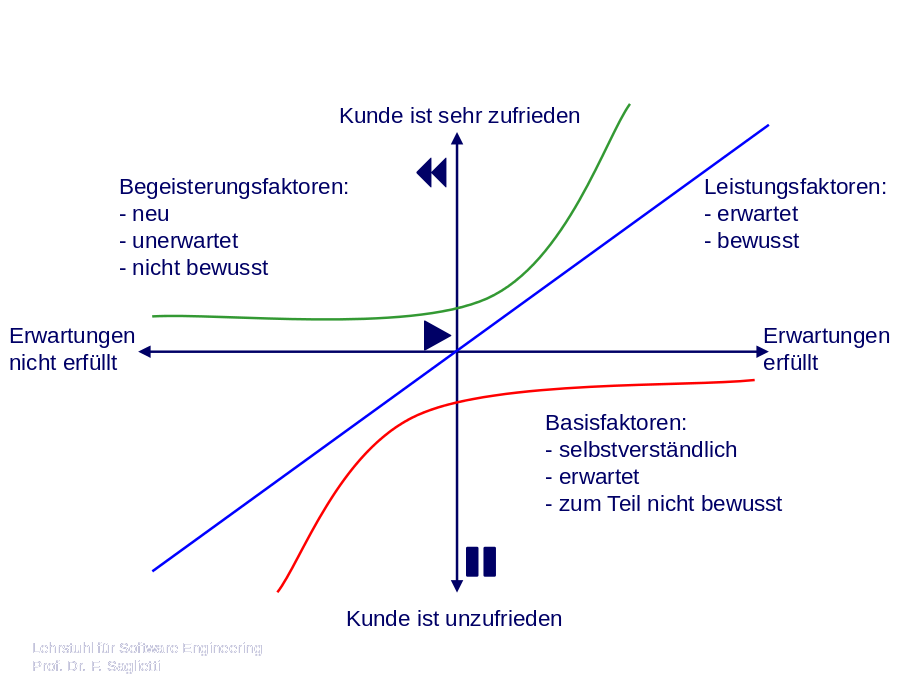
\includegraphics[scale=0.5]{./inc/Anforderungsspezifikation/ZufriedenheitUndErwartung.png}

























